\documentclass[sn-apa]{sn-jnl} % APA Reference Style 

\usepackage{graphicx}
\usepackage{amsmath,amssymb}
\usepackage[style=apa]{biblatex}
\addbibresource{my_bib.bib}

\begin{document}

\title[Supplementary Materials]{Supplementary Materials}

\maketitle

\section{Supplementary Note on Modality and Replication}

A recurring question in replication research is how to interpret differences
that result from pragmatic adaptations rather than intentional design choices.
In Ge et al. (2021), data were collected in two laboratories using different
hardware (Tobii TX300 in Hong Kong; EyeLink 1000 in the Netherlands). These
systems differ in sampling rate, calibration routines, and testing environments,
yet both sites were part of the same original study. This illustrates that even
within a single project, cross-site variability in equipment and context is
common. As \textcite{mcmanus2024} notes, replication studies will always involve
some deviations, and the critical requirement is that they are reported
transparently rather than ignored or over-interpreted as new methodological
conditions.

Our study followed this principle. We used web-based eye-tracking with
WebGazer.js and online recruitment via Prolific because these were the feasible
tools for collecting data. We did not design this as a test of “online versus
lab” methods, but as a pragmatic adaptation that allowed replication with
available resources. Web-based eye-tracking introduces limitations in temporal
precision relative to Tobii or EyeLink systems, but it also brings important
advantages: scalability, access to broader participant pools, and consistency
across testing sites. These trade-offs are consistent with broader open science
standards \parencite{goodman2016reproducibility} and with recent
field-specific guidelines for eye-tracking \parencite{godfroid2025reporting}. Moreover,
a growing body of research demonstrates that online eye-tracking is a viable
method for visual world studies when combined with careful calibration and
exclusion criteria \parencite[e.g.,][]{AOW}. 

A further point is that population differences almost always entail laboratory
differences. To study learners in different countries or speakers of different
languages, researchers must recruit across sites, each with its own hardware,
software, and testing conditions. Thus, methodological heterogeneity is
unavoidable when addressing cross-linguistic questions. The critical issue is
not whether every site, tool, or modality is identical, but whether the design
is faithfully reproduced and reported in sufficient detail for evaluation
\parencite{mcmanus2024}. Following prior work on online VWP experiments,
including \textcite{AOW}, our study demonstrates that replication can
preserve design fidelity while adapting pragmatically to new platforms. In this
sense, the move online should be understood as a practical decision, not a theoretical manipulation, and one that is consistent with the broader reality of replication in applied linguistics and psycholinguistics.


\section{Supplemental Materials: Frame Rate Distribution}

\noindent
Supplemental Materials Figure~\ref{fig:frame_rate} shows the distribution of effective frame rates across participants. Data were collected using 
WebGazer.js embedded in Gorilla, with participants’ own webcams. Because hardware could not be standardized (e.g., webcam model, screen size, or viewing 
distance), we instead report observable sampling characteristics. The shaded grey region marks the 5~Hz cutoff used for exclusion. Individual points (black) 
represent trial-level frame rates, red points show mean frame rate per participant, and the blue line indicates the overall mean across participants. This visualization illustrates that, while variability is inherent in online testing, most participants recorded above the cutoff and contributed usable data.

\begin{figure}[h]
    \centering
    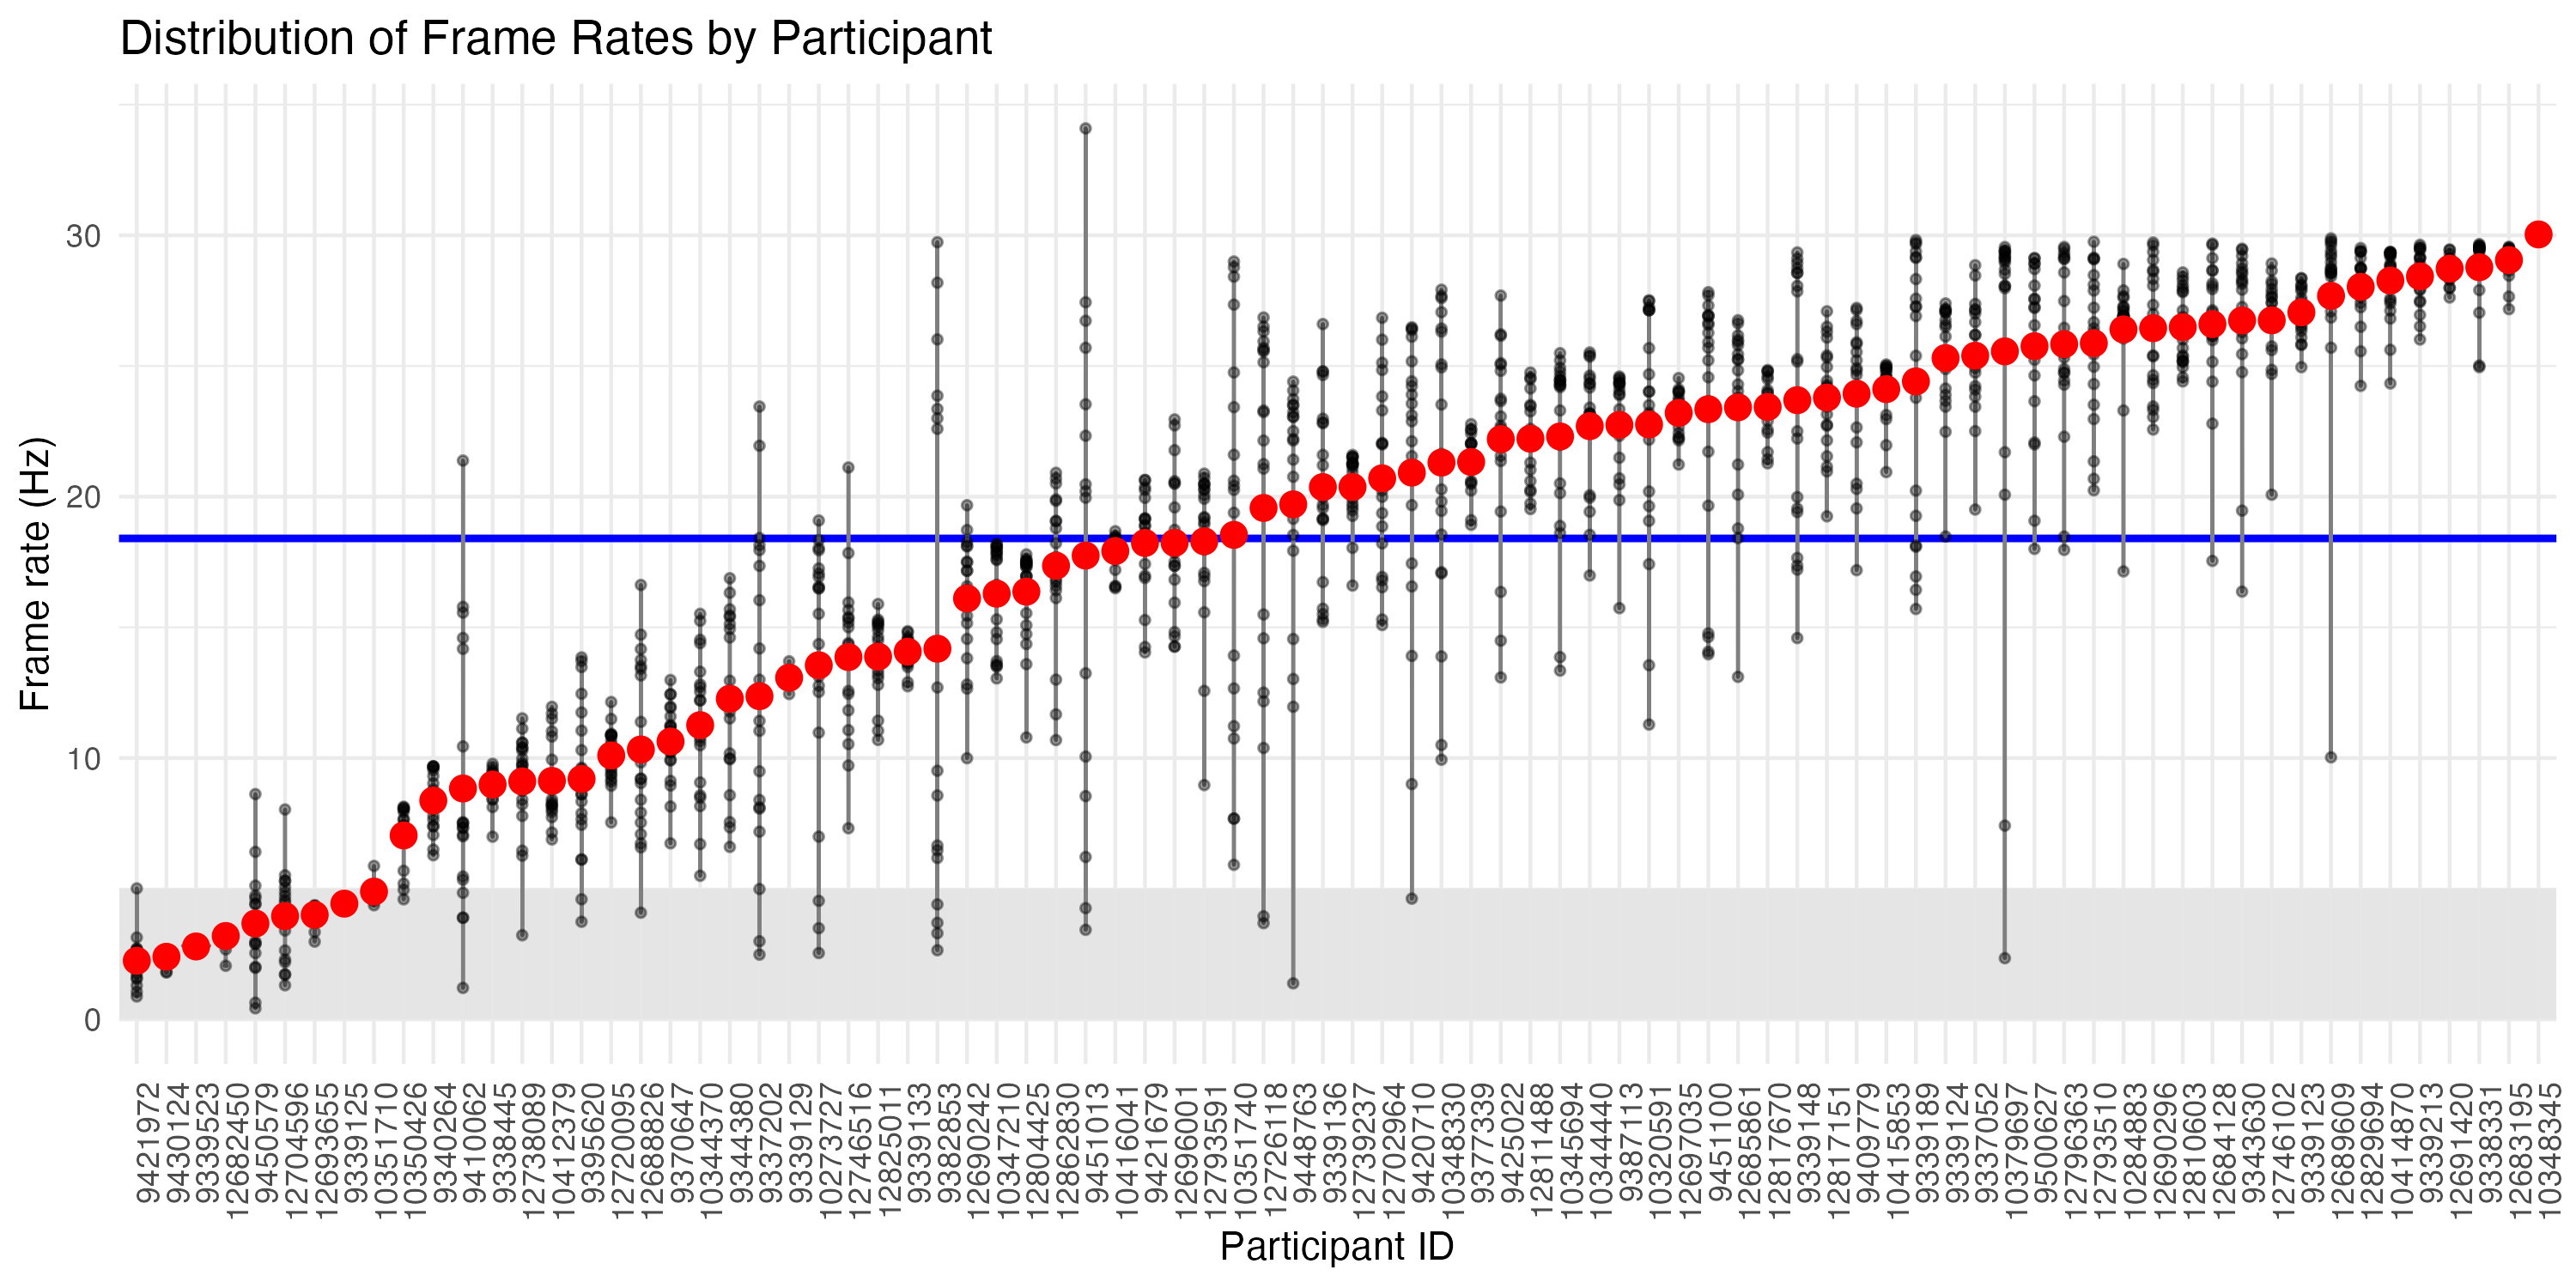
\includegraphics[width=\textwidth]{viz/fr.png}
    \caption{Distribution of effective frame rates across participants. Grey 
    shading marks the 5~Hz cutoff used for exclusion. Black points represent 
    trial-level frame rates, red points indicate participant means, and the 
    blue line shows the overall mean.}
    \label{fig:frame_rate}
\end{figure}

This style figure was inspired by-  \cite{AOW}. 

\section{Results}

\subsection{Interaction Analysis for Acoustic Cue Integration}

This additional analysis as shown in the right side of figure \ref{fig:analysis_3_plot} of the main paper, we investigated how different acoustic cues influence eye-fixations during word recognition. To do this, we built four mixed-effects models, two for each stress type at syllables 1 and 2, each with identical model structures. For both antepenultimate and penultimate models, target looks were used as the dependent variable with the four scaled measurements of the auditory stimuli (syllable-pitch, syllable-amplitude, syllable-spectral tilt, and syllable-duration) and their interactions. Additionally, \textit{word} and \textit{participant} were given random intercepts. Models with participant randome intercepts did not converge so we simplified to word only random intercepts. Following this, all models started with maximal models and were reduced using a backward stepwise selection procedure. 

The backward stepwise selection procedure began with the full model, which included all main effects and their interactions. Non-significant items were removed starting with the highest-order interactions, based on the significance levels from Wald z-tests. Each step involved refitting the model without the least significant main effect or interaction and comparing the fit of the reduced model to the previous model using AIC. The process continued until the removal of any additional terms resulted in a significant increase in AIC, indicating a poorer fit to the data. This method ensures that the final models were parsimonious, retaining only those predictors that contribute significantly to explaining the variance in target looks. While \cite{Sulpizio_McQueen_2012} confirmed analyses with reverse regression, their primary analysis focused on correlations between variables and eye-fixations. \hl{We also did a secondary analysis that includes interactions between speech cues that can be found in our online work\_flow on OSF, which was designed to allow us to capture more subtle variations across target fixations for Italian word stress. Results can be found in right figure \ref{fig:analysis_3_plot}


For the antepenultimate syllable 1 model, higher pitch led to fewer looks to the target ($\beta = -0.21$, \textit{SE} = 0.07, \textit{z} = -3.01, $p = 0.003$). Additionally, two interactions were found. First, when pitch and amplitude were both high, more looks were directed at the target ($\beta = 0.20$, \textit{SE} = 0.08, \textit{z} = 2.39, $p = 0.02$). Similarly, when both pitch and duration were higher, there were more looks to the target ($\beta = 0.20$, \textit{SE} = 0.07, \textit{z} = 2.62, $p = 0.009$).

In the antepenultimate syllable 2 model, both higher pitch ($\beta = -2.09$, \textit{SE} = 0.60, \textit{z} = -3.48, $p < 0.001$) and longer duration ($\beta = -1.25$, \textit{SE} = 0.48, \textit{z} = -2.58, $p < 0.01$) led to fewer looks at the target. When these two cues (higher pitch and longer duration) were combined, even fewer looks were directed at the target ($\beta = -1.60$, \textit{SE} = 0.61, \textit{z} = -2.62, $p = 0.009$).

For the penultimate syllable 1 model, no significant main effects were found. However, an interaction between spectral tilt and pitch ($\beta = -0.26$, \textit{SE} = 0.10, \textit{z} = -2.61, $p = 0.009$) suggested that higher tilt and pitch together led to fewer looks at the target. Additionally, when pitch and duration were both higher, more looks were directed at the target ($\beta = 0.20$, \textit{SE} = 0.06, \textit{z} = 3.13, $p = 0.002$).

In the penultimate syllable 2 model, higher amplitude led to more looks at the target ($\beta = 0.66$, \textit{SE} = 0.21, \textit{z} = 3.13, $p = 0.002$), while longer duration led to fewer looks at the target ($\beta = -0.30$, \textit{SE} = 0.12, \textit{z} = -2.53, $p = 0.01$). Several interactions were found: when amplitude and pitch were both high, there were fewer looks at the target ($\beta = -0.35$, \textit{SE} = 0.14, \textit{z} = -2.50, $p = 0.01$), and similarly, when amplitude and duration were both high, fewer looks were directed at the target ($\beta = -0.47$, \textit{SE} = 0.16, \textit{z} = -2.96, $p = 0.003$). However, when spectral tilt and pitch were both high, more looks were directed at the target ($\beta = 0.20$, \textit{SE} = 0.09, \textit{z} = 2.35, $p = 0.02$), and when pitch and duration were both high, more looks were directed at the target ($\beta = 0.26$, \textit{SE} = 0.09, \textit{z} = 2.99, $p = 0.003$).

\end{document}
